\documentclass[aspectratio=43]{beamer}

\usepackage[T1]{fontenc}
\usepackage[utf8]{inputenc}
\usepackage[english]{babel}
\usepackage{pgfplots}
\pgfplotsset{compat=newest}
\usepackage{booktabs}
\usepackage{siunitx}

% Latin Modern
\usepackage{lmodern}
% Verdana font type
%\usepackage{verdana}
% Helvetica
%\usepackage{helvet}
% Times (text and math)
%\usepackage{newtx, newtxmath}

%\usetheme[department=compute]{DTU}

\title[DTU Templates]{02445 \\ Statistical evaluation  \\ of artificial intelligence systems}
\author{Nikolaj S. Povlsen \\ Rasmus J. Pedersen}
\institute{Technical University of Denmark (DTU)}
\date{\today}
	
\newcommand{\tabitem}{{\color{dtured}$\bullet$} }

\begin{document}
\frame{
	\maketitle
}




\frame{
	\frametitle{Project 2}
	\begin{block}{Choosing between Olsen P and DGT measurements}
		\begin{itemize}
			\item Evaluating models
			\item Testing for significance
			\item Analyzing residuals
		\end{itemize}
	\end{block}
	\begin{block}{Does the amount of bio-available phosphorous influence the harvest yield?}
	
	\end{block}
}

\frame{
	\frametitle{Choosing between Olsen P and DGT measurements}

		\begin{figure}[H]
			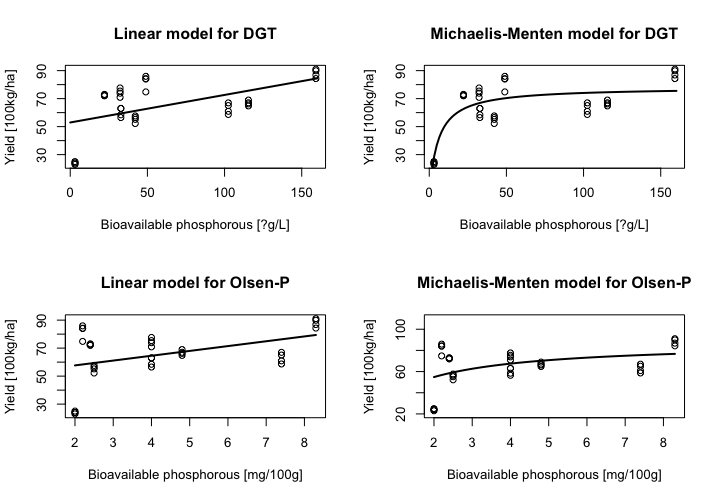
\includegraphics[width=\linewidth]{linearnonlinear.png}
		\end{figure}
}





\frame{
	\frametitle{Choosing between Olsen P and DGT measurements}
	
	\begin{block}
		
		
		\begin{table}
			\tiny
			\begin{tabular}{lcccc}\toprule [1.5pt]
				\textbf{Model}                & \multicolumn{1}{l}{\textbf{Linear DGT}} & \multicolumn{1}{l}{\textbf{Linear Olsen-P}} & \multicolumn{1}{l}{\textbf{Non-linear DGT}}  & \multicolumn{1}{l}{\textbf{Non-linear Olsen-P}}         \\ \midrule
				\textbf{Std squared error} & 15.37        & 16.55             & 10.58             &    16.33           \\\midrule
				\textbf{p-values}   & DGT = 0.000685       & Olsen-P = 0.0103      & \begin{tabular}[c]{@{}c@{}}Alpha = 2e-16\\ Beta = 0.0014\end{tabular} & \begin{tabular}[c]{@{}c@{}}Alpha = 1e-9\\ Beta = 0.0432\end{tabular}\\
				\bottomrule[1.25pt]
			\end{tabular}
		\end{table}
		
		
	\end{block}
}

\frame{
	\frametitle{Choosing between Olsen P and DGT measurements}
	\begin{table}[H]
		\small
		\begin{tabular}{lrcr}\toprule[1.5pt]
			\textbf{Paired t-test between:}                          & \multicolumn{1}{l}{\textbf{t-statistic}} & \multicolumn{1}{l}{\textbf{df}} & \multicolumn{1}{l}{\textbf{p-values}} \\\midrule
			Non-Linear DGT - Non-linear Olsen-P & -2.694                                   & 35                              & \textbf{0.011}                                \\\midrule
			Non-Linear DGT - Linear Olsen-P     & -2.481                                   & 35                              & 
			\textbf{0.018}                                \\\midrule
			Non-Linear DGT - Linear DGT         & -2.381                                   & 35                              & \textbf{0.023}                                 \\\midrule
			Linear DGT - Linear Olsen-P         & -1.874                                   & 35                              & 0.069                                 \\\midrule
			Linear DGT - Non-linear Olsen-P     & -1.590                                   & 35                              & 0.12                                  \\\midrule
			Linear Olsen-P - Non-linear Olsen-P & 0.3065                                   & 35                              & 0.76                      \\
			\bottomrule[1.25pt]           
		\end{tabular}
	\end{table}
}

\frame{
	\frametitle{Residuals from linear and non-linear DGT measurements}
	
	\begin{figure}[H]
		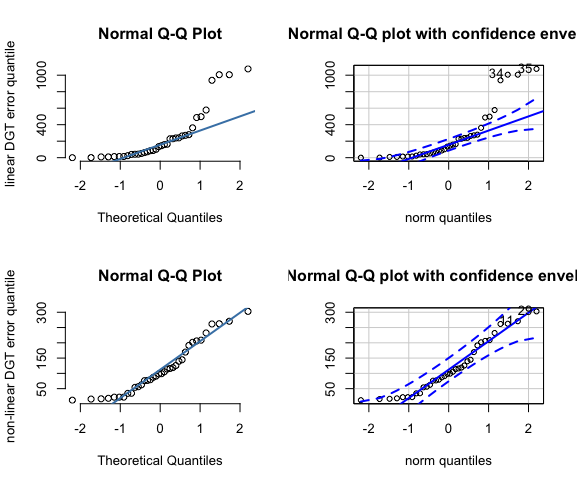
\includegraphics[width=.9 \linewidth]{qqplot.png}
	\end{figure}
}





%%%% Next project
\frame{
	\frametitle{Project 1}
	\begin{block}{Classifying 3D motions}
		\begin{itemize}
			\item Comparing models
		\end{itemize}
	\end{block}
	\begin{block}{Does the experiment influence the motion}
		\begin{itemize}
			\item Test statistics
			\item PCA
			\item $T^2$
		\end{itemize}
		
	\end{block}
}

\frame{
	\frametitle{Resuts}
	\begin{block}{Model accuracy}
		\begin{table}
			\begin{tabular}{ c c}\toprule[2pt]
				\bf Model  & \bf CI of Generalization Accuracy \\\midrule[1.5pt]
				ANN  & $0.708 \pm 0.0078$  \\\midrule
				KNN  & $0.644 \pm 0.0066$ \\
				\bottomrule[1.25pt]
			\end {tabular}
		\end{table}
	\end{block}
	\begin{block}{Paired t-test}
		\begin{table}
			\begin{tabular}{ c c c}\toprule[1.5pt]
				\bf Test  & \bf Test Statistic & \bf p-value \\\midrule[1.5pt]
				Paired t-test  & $10.934$ &  $8e-12$ \\
				\bottomrule[1.5pt]
			\end {tabular}
		\end{table}
	\end{block}

}


\frame{
	\frametitle{Testing for normally distributed variables}
	\centering
	\begin{figure}

		\includegraphics[width=0.9\linewidth]{multiVar.png}
	\caption{Two univariate variables forming a multivariate distribution. Left pane shows approximately a multivariate normally distribution, the right does not.}
	\end{figure}
}
\frame{
	\frametitle{Central Limit Theorem }
	\centering	\LARGE \color{red} Equals a 90\% reduction in sample size.

}
\frame{
	\frametitle{PCA }
	\large But 9 principal components explain 82\% of the variance
		\begin{figure}[H]
		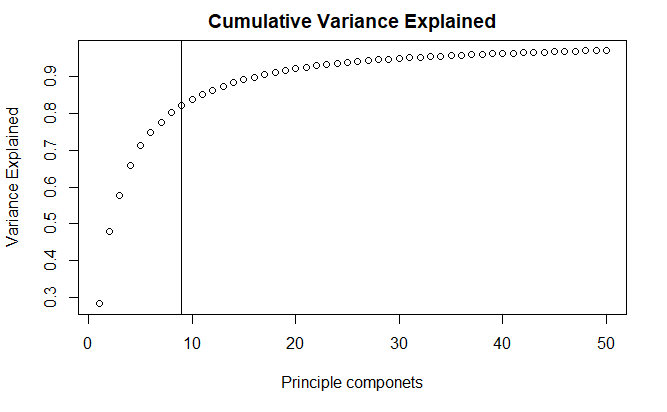
\includegraphics[width=\linewidth]{variance_explained.png}
	\end{figure}
	
}

\frame{
	\frametitle{$T^2$}
	\Large 5 out of 120 pairs of tests were not significant
	\centering
	\begin{table}
		\small
		\begin{tabular}{cc}\toprule[1.5pt]
			\textbf{Experiment pair} & \textbf{p-value} \\\midrule[1.25pt]
			1, 4         	& 0.137            \\\midrule
			4, 7  		& 0.177            \\\midrule
			7, 10           	& 0.278            \\\midrule
			5, 8        	& 0.0855           \\\midrule
			6, 9      	& 0.162           \\\bottomrule[1.25pt]
		\end{tabular}
	\end{table}
	
}

\frame{
	\frametitle{The experiments}
	\centering
	\LARGE

\begin{table}[]
	\begin{tabular}{l|lll}
		& S                      & M  & T  \\ \hline
		15.0 cm & \color{violet}1                      & 2  & 3  \\ 
		22.5 cm & \textbf{\color{violet}4} & \color{red}5  & \color{orange}6  \\
		30.0 cm & \textbf{\color{blue}7} & \color{red}8  & \color{orange}9  \\ 
		37.5 cm & \color{blue}10                     & 11 & 12 \\
		45.0 cm & 13                     & 14 & 15
	\end{tabular}
\end{table}

}

\end{document}